\section{Introduction}
\label{sec:intro}
\subsection{Motivation}
A long time ago, a scientist was looking at galaxies far far away. 
They noticed that different galaxies have different morphologies that can be split into two main categories: spiral and elliptical. 
The differences between them are fairly obvious when looking at images: spiral galaxies are disk shaped and have curved arms extending out from the centre, while elliptical galaxies are shaped like a three dimensional blob that is brighter in the middle (Figure \ref{fig:tuningfork}). 

\begin{figure}[h!]
	\centering
	\captionsetup{justification=centering,width=.8\linewidth}
	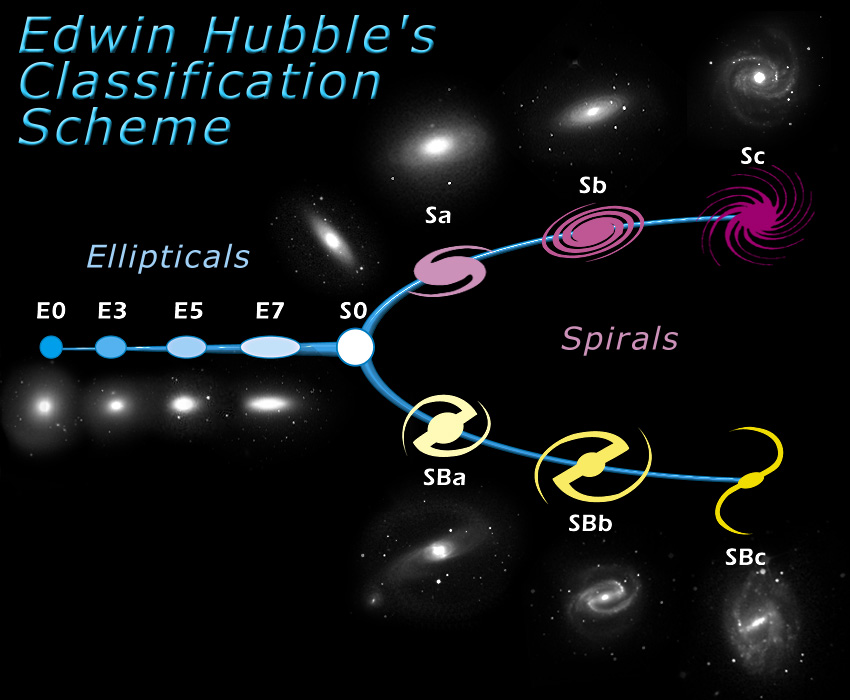
\includegraphics[scale=0.7]{Figures/TuningFork.jpg}
	\caption{Edwin Hubble's 'Tuning Fork' classification scheme. Galaxies are classified into two main categories, spiral and elliptical, with further sub-classifications representing minute changes not discussed in this report \cite{TuningFork}.}
	\label{fig:tuningfork}
\end{figure}


There are however many differences between the two galaxy morphologies that are not as glaringly obvious.  
For example, Spiral galaxies tend to be bluer than their elliptical cousins. 
Dense spiral arms are the birthplace of new stars, which excite gas around them and cause it to glow a blue colour. 
Elliptical galaxies lack the gas and dust required to form new stars, and therefore tend to be redder.

Classifying galaxies based on their morphology has an enormous impact on research in many fields of astronomy, including things from galactic dynamics to actually determining the age of a galaxy!
That last point may sound skeptical, however consider the event of galaxy collisions.
When two galaxies of any type collide, they eventually form a large elliptical galaxy. 
Elliptical galaxies are much more common near the centre of galaxy clusters for this reason, and can be many times larger than their spiral counterparts.
This is why scientists see more spiral galaxies as we look deeper into space - because it is analogous to looking further back in time where fewer spiral galaxies had time to collide and form ellipticals. 


Humans can easily distinguish between the two morphologies by just looking at the galaxy images. 
However there is one major problem in this field of research that is rather unexpected - we have too much data available to look through and separate! 
The Sloan Digital Sky Survey is one of the newer collection surveys that is starting to monopolize the field. The newest SDSS data release has a list of over 200,000,000 individual galaxies across more than one third of the night sky\cite{SDSS}!

\subsection{Approach}
This is where data science comes in!
We first performed Logistic regression on the data, specifically on the average flux value of each image channel. 
This was to see if there was any obvious relationship between the colour of the galaxy and its morphology. 
We then trained a neural network to classify galaxy images as spiral or elliptical.
If successful, a convolutional neural network (CNN) should be able to classify galaxies much faster than humans, with comparable accuracy.












